\documentclass[11pt]{article}

\usepackage[utf8]{inputenc}
\usepackage[T1]{fontenc}

\usepackage[a4paper, left=2cm, right=2cm, top=3.5cm, bottom=3.5cm]{geometry}
\usepackage[french]{babel}

% Paragraph spacing
\setlength{\parskip}{1em}

% Fancy headers
\usepackage{fancyhdr}

% Captions for subfigures
\usepackage{subcaption}

% Code highlighting
\usepackage{minted}

% Footnote inside a caption
\usepackage{fnpos}
\usepackage{ftnxtra}

% Maths
\usepackage{amsmath}
\usepackage{amssymb}

% Todo notes
\usepackage{todonotes}

% Table of contents for bibliography
\usepackage[nottoc]{tocbibind}

% Inline monospace font
\def\code#1{\texttt{#1}}

% Figures
\usepackage{graphicx}

% Draw figures
\usepackage{tikz}

% Tikz node rotation
\usetikzlibrary{positioning}

% Turing machine
\usetikzlibrary{chains,fit,shapes}

% Usage: \rotnode[options]{rotation}{text}
\newcommand\rotnode[3][]{%
    \node [#1, opacity=0.0] (tmp) {#3};
    \node [draw, rotate around={#2:(tmp.center)}] at (tmp) {#3};
}

% Clickable links
\usepackage{hyperref}

% Table of contents depth
\setcounter{tocdepth}{2}

% Inline code
\usepackage{listings}
\usepackage{color}

\title{Systèmes d'exploitation : virtualisation}

\author{William SCHMITT}
\date{2018-2019}

\begin{document}
\maketitle

\section{Niveaux de virtualisation}

\subsection{Virtualisation au niveau hardware}
\begin{itemize}
    \item IBM mainframe
    \item Intel : \begin{itemize}
        \item 4 user
        \item 3
        \item 2
        \item 1 kernel
        \item -1 mode hyperviseur
    \end{itemize}
\end{itemize}

\subsection{Virtualisation au niveau OS}

\subsubsection{OS complets}
\begin{figure}[ht]
    \centering
    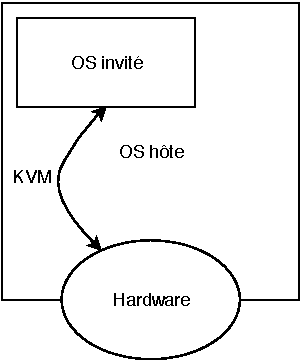
\includegraphics{img/c3-kvm.pdf}
\end{figure}
On simule un OS complet dans un OS hôte, des mécanismes comme KVM permettent l'interaction entre OS invité et matériel.

\subsubsection{Containers}
\begin{figure}[ht]
    \centering
    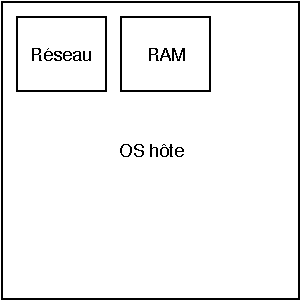
\includegraphics{img/c3-container.pdf}
\end{figure}

Une autre façon de virtualiser est de privatiser (ou dupliquer) des parties de l'OS : c'est les systèmes de containers tels que \textbf{docker}. On peut avoir des systèmes de fichiers différents, et donc des bibliothèques différentes.

\subsubsection{Jails}
\begin{figure}[ht]
    \centering
    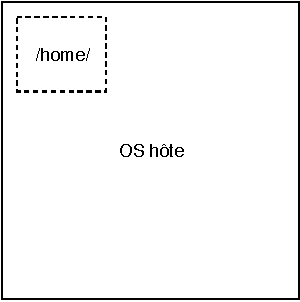
\includegraphics{img/c3-jails.pdf}
\end{figure}

Un seul OS, les processus ont l'impression de tourner sur un OS normal, mais tournent dans un overlay d'un bout de l'OS : les fichiers peuvent par exemple être supprimés.

\subsection{Virtualisation au niveau processus}

Java tourne dans la JVM. Les mêmes mécanismes sont mis en oeuvre dans python ou perl : des \textit{just-in-time} sont utilisés pour traduire le code utilisé dans la JVM vers des instructions tilisables par la machine.

D'autres langages, comme Julia qui ressemble à Python, n'utilisent pas ces mécanismes : Julia est compilé avec clang au lancement de l'exécutable.

\end{document}